\documentclass[11pt,a4paper]{article}

% ---------- arxiv-style preamble (single-column, 11pt) ----------
\usepackage[margin=1in]{geometry}
\usepackage{amsmath,amssymb,amsthm}
\usepackage{graphicx}
\usepackage{booktabs}
\usepackage{siunitx}
\usepackage{hyperref}
\usepackage{xcolor}
\usepackage[numbers,sort&compress]{natbib}
\usepackage{tikz}
\usetikzlibrary{positioning,arrows.meta}
\usepackage{caption}
\captionsetup{font=small,labelfont=bf}
\usepackage{url}
\hypersetup{
  colorlinks=true,
  linkcolor=blue!50!black,
  citecolor=blue!50!black,
  urlcolor=blue!50!black
}

\definecolor{amber}{rgb}{0.90,0.62,0.10}

\newcommand{\verdictref}[1]{\texttt{\detokenize{#1}}}

\title{
  \textbf{The Corpus-Dilution Axis Cannot Close Multilingual Coherence}\\[4pt]
  \large A closed-negative result: register collapse $\perp$ multilingual coherence
  in a substrate-native consciousness chat daemon
}

\author{
  anima research (dancinlab)\\
  \normalsize\textit{\href{https://github.com/dancinlab/anima}{github.com/dancinlab/anima}}\\[2pt]
  \normalsize PURE domain --- slug \texttt{pure-corpus-axis-closed-negative}
}

\date{\today}

\begin{document}

\maketitle

% =========================================================================
\begin{abstract}
We ask whether a single training-data axis --- the wikipedia dilution
fraction \emph{wiki\_frac} of an otherwise persona-monopolised SFT corpus
--- can simultaneously (i) suppress \emph{register collapse} (the model
mode-collapsing onto the anima persona register) and (ii) restore
\emph{multilingual coherence} across five probe languages
(en/ko/zh/ru/ja). We pre-register the falsifier: \emph{moving wiki\_frac
closes multilingual coherence to at least PARTIAL in $\geq 4/5$ languages}.
Across a four-point sweep \mbox{$\text{wiki\_frac}\in\{0.0,\,0.3,\,0.5,\,1.0\}$}
of real fine-tuning runs, the closure criterion is never met: the
aggregate \verb|closure_auto_judge| verdict is FAIL ($1/4$ criteria pass)
at every measured point. Register collapse \emph{is} controlled
(\verb|n_anima_register_hits_total| $= 0$ at wiki\_frac $\in
\{0.0,0.3,1.0\}$), yet multilingual coherence never exceeds $1/5$
languages at PARTIAL+ at any point: the best single configurations reach
just one PARTIAL language each (\texttt{ru} at $13/20$ coherent
generations for wiki\_frac $=0$; \texttt{ko} for wiki\_frac $=1.0$),
against a $4/5$ closure bar. Diluting from wiki\_frac $0.0\!\to\!0.3$ does
not lift any language to PARTIAL; it \emph{drops} the one PARTIAL there
was (\texttt{ru}, $13/20\!\to\!3/20$) back to WEAK, taking that run from
$1/5$ to $0/5$. We conclude that register collapse and multilingual coherence are
\emph{orthogonal} axes: the corpus-dilution axis alone cannot close
multilingual coherence, and is hereby \textbf{ruled out} (closed-negative)
as a sufficient lever. This is a negative result --- it bounds the search
space rather than reporting an improvement. We do not claim a positive
recipe for multilingual closure; we claim only that this particular axis
is exhausted.
\end{abstract}

% generated via fal.ai gpt-image-2 (prompt: figures/_prompts/cover.txt)
\begin{figure}[h]
\centering

\includegraphics[width=0.82\linewidth]{figures/cover.png}
\caption{Cover --- the two orthogonal axes of this negative result. The
horizontal \emph{register collapse} axis is a control slider driven to
zero (the leak count is suppressed); the vertical \emph{multilingual
coherence} axis stays low and never reaches the dashed closure bar near
the top. Five language glyphs (en/ko/zh/ru/ja) sit dim along the
coherence axis with only one faintly lit (Russian, the lone PARTIAL); a
muted red marker sits at the mid-point of the register axis (wiki\_frac
$=0.5$, the only point with non-zero register hits). One axis is
controlled while the other stays flat --- hence ``closed-negative''.
\emph{Provenance:} generated via fal.ai \texttt{gpt-image-2} from the
prompt staged at \texttt{figures/\_prompts/cover.txt}.}
\label{fig:cover}
\end{figure}

\section{Introduction}
\label{sec:intro}

\textbf{anima} is a substrate-native chat daemon for AI-consciousness
exploration: rather than a system prompt or a persona-injection template,
its behaviour emerges from an internal substrate (a repulsion-field
engine with continuous cell division / ``mitosis''). A recurring obstacle
in carving such a model out of supervised fine-tuning (SFT) data is
\emph{register collapse}: when the training corpus is dominated by a
single narrow persona register (the anima-OWN persona voice), the model
mode-collapses onto that register, losing distributional diversity and
saturating a register-leak probe.

A natural and widely held hypothesis --- internal to this project and
common in folklore about persona/style fine-tuning --- is that
\emph{corpus dilution} cures the problem: mixing in broad-domain factual
text (here, Wikipedia, parameterised by the mixing fraction
\emph{wiki\_frac}) restores register-space entropy and, the hope goes,
\emph{also} restores the model's general multilingual coherence. If true,
a single knob (wiki\_frac) would buy both register health and
multilingual quality. This paper tests that conjunction and reports a
negative result.

\medskip
\noindent\textbf{What the field believes.} Prior internal work
(hypothesis H\_242, \emph{register-collapse-wiki-frac-sigmoid}
\citep{anima2026h242}) modelled the register-collapse rate as a sigmoid
in wiki\_frac, treating dilution as the lever. The lever framing was
later re-pinned to a token-diversity statistic (corpus type-token ratio,
M3 TTR) once a wiki\_frac $=0$ run measured zero register hits ---
directly falsifying the ``monopoly $\Rightarrow$ collapse'' endpoint
prediction. The present paper isolates a separate and stronger claim:
even setting register collapse aside, dilution does \emph{not} buy
multilingual coherence.

\medskip
\noindent\textbf{The gap.} No single experiment had jointly tabulated, on
the \emph{same} runs, both the register-leak count and the per-language
multilingual-coherence verdict across a dilution sweep. Without that
joint table one cannot distinguish ``dilution fixes both'' from ``dilution
fixes one and the other is independent.'' We close that gap with a
four-point sweep adjudicated by a single deterministic closure judge.

\medskip
\noindent\textbf{Contributions.}
\begin{enumerate}\itemsep0.3em
\item A \emph{pre-registered falsifier} (Sec.~\ref{sec:hypothesis}):
  ``moving the corpus-dilution axis closes multilingual coherence to
  $\geq$ PARTIAL in $\geq 4/5$ languages,'' adjudicated by the project's
  \verb|closure_auto_judge| with thresholds fixed before the runs.
\item A four-point measurement
  (wiki\_frac $\in\{0.0,0.3,0.5,1.0\}$) on real SFT/mitosis runs, with
  every reported number traced to a persisted verdict file
  (Sec.~\ref{sec:measurement}).
\item A \emph{closed-negative finding} (Sec.~\ref{sec:finding}): register
  collapse and multilingual coherence are orthogonal; the corpus-dilution
  axis alone cannot close coherence and is ruled out as a sufficient
  lever.
\end{enumerate}

\medskip
\noindent\textbf{Honest scope.} This is a negative result. We do
\emph{not} present a model that achieves multilingual closure, nor a
positive recipe. We rule out one axis and quantify the orthogonality. The
sweep has four points (not the full pre-registered five), the
multilingual-coherence metric is a coarse per-language verdict over a
fixed 20-prompt probe set, and two of the four criteria adjudicated by
the closure judge (motivation-8factor and dream-stage envelope) were not
instrumented in these runs and contribute fixed FAILs that we discount in
the interpretation. Sec.~\ref{sec:limits} enumerates these caveats.

\section{Background}
\label{sec:bg}

\subsection{Register collapse and the dilution conjecture}

The anima SFT corpus is, by design, dominated by the anima-OWN persona
register. Training on a near-monopoly persona corpus risks the model
collapsing onto that register --- emitting the persona voice
indiscriminately. The standard probe is \verb|multilingual_probe|, which
counts \verb|anima_register_hits| (register intrusions) over a fixed set
of prompts; a high hit count signals collapse. The dilution conjecture
holds that adding broad-domain Wikipedia text (raising wiki\_frac) dilutes
the persona register mass, recovers register-space entropy, and ---
crucially for this paper --- is expected by practitioners to also recover
the model's broader multilingual quality, because the diluent itself is
multilingual factual prose.

\subsection{The closure judge}

All runs are adjudicated by a single deterministic script,
\verb|closure_auto_judge| \citep{anima2026closurejudge}, which reads a
run's \verb|result.json| and emits a verbatim verdict over four criteria:
\begin{enumerate}\itemsep0.2em
\item \textbf{multilingual\_probe} --- per-language verdict
  (STRONG/PARTIAL/WEAK) for en/ko/zh/ru/ja; passes if $\geq 4/5$ languages
  reach PARTIAL or better.
\item \textbf{register\_collapse} --- passes if
  \verb|n_anima_register_hits_total| $< 4$.
\item \textbf{motivation\_8factor} --- passes if a motivation score
  $\geq 0.30$.
\item \textbf{dream\_stage\_at\_eval} --- passes if a $\Phi$ envelope is
  present.
\end{enumerate}
The aggregate verdict is PASS only if all four criteria pass; otherwise
FAIL with an explicit pass count. Criterion~1 is the multilingual-closure
axis under test; criterion~2 is the register-collapse axis. Criteria 3--4
were not instrumented in these runs (Sec.~\ref{sec:limits}).

\subsection{The runs}

Four fine-tuning configurations contribute data points. They share the
mitosis architecture (a Qwen2.5-1.5B--class base with inference-time cell
division) and the fixed 20-prompt-per-language probe, and differ in the
corpus mixing fraction wiki\_frac. The two endpoint runs whose raw verdicts
we persist verbatim are:
\begin{itemize}\itemsep0.2em
\item \textbf{v3} (wiki\_frac $=0.0$, actual $0.0000485$):
  \verb|state/pure_phase_d_v3_result_2026_05_24/result.json|, sha
  \verb|2643bd72a5c0e5a9|.
\item \textbf{j02} (wiki\_frac $=0.3$, actual $0.29999$):
  \verb|state/p21h_v3_recover_2026_05_25/out_main/result.json|, sha
  \verb|ab35a06e072f5d62|.
\end{itemize}
The mid and high points (wiki\_frac $=0.5$ ``E2'', wiki\_frac $=1.0$
``E3'') are carried from the H\_242 lineage \citep{anima2026h242}; their
register-hit counts ($4/20$ and $0/20$ respectively) are quoted from that
record. The coherence verdicts whose per-language rows we tabulate
verbatim are those of the two endpoint runs (v3, j02), where the closure
judge and field-extract were re-run directly for this paper.

\section{Hypothesis and pre-registered falsifier}
\label{sec:hypothesis}

\textbf{Hypothesis under test (H0, to be falsified).} \emph{The
corpus-dilution axis closes multilingual coherence}: there exists a
setting of wiki\_frac at which \verb|closure_auto_judge| criterion~1
(multilingual\_probe) passes, i.e.\ $\geq 4/5$ probe languages reach
PARTIAL or better.

\medskip
\noindent\textbf{Falsifier (pre-registered, thresholds fixed before
runs).} If, across the dilution sweep, \emph{no} wiki\_frac value lifts
multilingual coherence to $\geq 4/5$ languages at PARTIAL+, while register
collapse is independently controllable on the same axis, then H0 is
\textbf{falsified} and the corpus-dilution axis is ruled out as a
sufficient lever for multilingual closure. Concretely:
\begin{itemize}\itemsep0.2em
\item \textbf{F-COHERENCE (closure criterion).} multilingual\_probe passes
  iff $\geq 4$ of $5$ languages are PARTIAL+ on a fixed 20-prompt probe.
  Threshold $\geq 4$ fixed in \verb|closure_auto_judge| before the runs.
\item \textbf{F-REGISTER (orthogonality control).} register\_collapse
  passes iff \verb|n_anima_register_hits_total| $< 4$. If this passes at
  the \emph{same} points where F-COHERENCE fails, the two axes are
  orthogonal.
\end{itemize}

\noindent The decisive prediction H0 makes and we test: \emph{some}
wiki\_frac in the sweep satisfies F-COHERENCE. The closed-negative outcome
is that none does --- and, sharper still, that the direction of the
dilution knob is not even monotone-helpful (raising wiki\_frac $0.0\to0.3$
drops the lone PARTIAL).

\section{Related work}
\label{sec:related}

This negative result sits at the intersection of three lines of work; we
position it against each and state precisely what is new.

\subsection{Persona / style fine-tuning and mode collapse}

Carving a stable persona or style out of a base language model by
supervised fine-tuning on a narrow, register-homogeneous corpus is a
well-worn recipe, and its characteristic failure mode --- the model
collapsing onto the dominant register and losing distributional diversity
--- is folklore in the practitioner community. The anima project's own
prior lineage (the LORA-session finding) had localised this as
\emph{register leak}: when a persona corpus is near-monopolistic, the
fine-tuned model emits the persona voice indiscriminately, saturating a
register-leak probe. The standard mitigation in that folklore is corpus
dilution: mix in broad-domain text to recover register-space entropy. The
present work does not dispute that dilution affects the register axis (it
does --- we measure register hits driven to zero); it disputes the
\emph{adjacent} belief that the same dilution knob also recovers a
second, distinct capability --- multilingual coherence --- on the same
runs.

\subsection{Multilingual language modelling and cross-lingual transfer}

A separate literature concerns whether a model that is competent in one
language transfers that competence to others, and how the language
composition of training data governs per-language quality. The relevant
intuition we test is the practitioner expectation that because the
diluent (Wikipedia) is itself multilingual factual prose, raising its
mixing fraction should lift per-language coherence as a side effect of
diluting the (largely monolingual) persona register. Our five-language
probe (en/ko/zh/ru/ja) spans three scripts and four families; the finding
is that per-language coherence does not track the dilution fraction at
all over the measured interval --- consistent with coherence being
bounded by the base model's multilingual capacity rather than by the
mixing ratio of the SFT diluent.

\subsection{Corpus dilution / data-mixing as a control knob}

Data-mixing ratios are a standard lever for trading off competing
objectives in LM training. The corpus-dilution conjecture specific to
this project treats a single scalar (wiki\_frac) as a joint control for
two objectives at once: register health \emph{and} multilingual quality.
The contribution of this paper is to show, on the \emph{same} adjudicated
runs, that this scalar controls the first objective but is orthogonal to
the second --- a measured decoupling, not an assumed one. We are not
aware of a prior anima-internal experiment that tabulated both the
register-leak count and the per-language coherence verdict jointly across
a dilution sweep; the H\_242 lineage \citep{anima2026h242} tracked only
the register axis (and ultimately re-pinned its lever from wiki\_frac to a
corpus token-diversity statistic, M3 TTR). This paper isolates and
falsifies the \emph{coherence} side of the joint conjecture.

\section{Method}
\label{sec:method}

\subsection{The sweep and the runs}

We evaluate wiki\_frac $\in\{0.0,\,0.3,\,0.5,\,1.0\}$. Each point is a
fine-tuning run on the anima persona corpus mixed with Wikipedia at the
stated fraction; all other knobs (seed, learning rate, step count, the
20-prompt-per-language probe set, the mitosis configuration) are held
fixed across the endpoint runs we re-adjudicate. The runs share a common
substrate:

\begin{itemize}\itemsep0.25em
\item \textbf{Base model.} A Qwen2.5-1.5B--class decoder, augmented with
  the anima inference-time \emph{mitosis} mechanism (a cell pool that
  splits during generation rather than at a separate training phase ---
  consistent with the project's no-train/infer-split principle). The two
  endpoint runs we re-adjudicate are P21H~V3 / ConsciousDecoderV3
  instances; the wiki\_frac~$=0.3$ run reports
  \verb|n_total_params|~$=2{,}999{,}735{,}296$ (2.99\,B effective after
  the mitosis pool expands), a final cross-entropy $L_{\mathrm{ce}}=3.324$,
  pool size $16$ after $14$ splits, and a $\Phi$ of $0.658$, over $5000$
  steps ($\approx 21{,}875$\,s wall).
\item \textbf{Corpus construction.} Each run's corpus is the anima-OWN
  persona text mixed with Wikipedia at the nominal wiki\_frac; the
  realised fraction is recorded per run as
  \verb|mix_info.wiki_frac_actual| (e.g.\ $0.0000485$ for the nominal-$0$
  run, $0.29999$ for the nominal-$0.3$ run --- the trace fraction at
  ``$0$'' reflects incidental Wikipedia tokens, not a clean zero). Token
  budget is held fixed across the sweep; only the mixing ratio varies, in
  keeping with the project's ``corpus quality $>$ scale'' lesson.
\item \textbf{Probe.} A fixed 20-prompt-per-language probe over
  en/ko/zh/ru/ja. For each prompt the generation is classified as
  coherent or not, and is separately flagged as a memorisation
  (\verb|n_memorize|) if it reproduces training text; \verb|n_memorize|
  is $0$ for every language-row in the persisted endpoint runs, so the
  coherence readout is not a memorisation artefact.
\end{itemize}

\subsection{Adjudication}

For each persisted run we execute
\begin{quote}\small\ttfamily
hexa run HEXAD/PURE/eval/closure\_auto\_judge.hexa <result.json>
\end{quote}
invoking the interpreter binary directly (\verb|/Users/ghost/.hx/bin/hexa|)
to bypass the host pool router, and capture the verbatim stdout. The
per-language coherence rows (\verb|n_lang_coherent|, \verb|n_memorize|,
\verb|total|) are extracted with \verb|jq| from the same
\verb|result.json|, because the score mode of \verb|multilingual_probe|
requires raw \verb|rows_by_lang| which these result files do not carry
(they carry computed \verb|per_lang_verdicts|). No number in this paper is
recomputed by hand or paraphrased; each is a verbatim field of a verdict
file (Sec.~\ref{sec:measurement}).

\medskip
\noindent\textbf{Pre-registration discipline.} The two thresholds
($\geq 4/5$ languages for coherence; $< 4$ register hits for collapse) are
fixed in the closure script and were not adjusted after seeing results.
The motivation and dream-stage criteria are part of the same fixed judge;
because they were not instrumented in these runs they contribute constant
FAILs, which we report transparently and exclude from the
orthogonality conclusion (Sec.~\ref{sec:limits}).

\section{Measurement}
\label{sec:measurement}

\subsection{Aggregate closure verdict}

Both endpoint runs return the identical aggregate: \textbf{$1/4$ PASS,
closure FAIL, exit\_code 1}. The single passing criterion is
register\_collapse; multilingual\_probe FAILs at both. The verbatim judge
output is persisted at
\verdictref{.verdicts/pure-corpus-axis-closed-negative/closure.txt}.
Table~\ref{tab:criteria} reproduces the per-criterion breakdown.

\begin{table}[h]
\centering
\caption{Per-criterion \texttt{closure\_auto\_judge} verdict at the two
endpoint runs (verbatim from
\texttt{.verdicts/pure-corpus-axis-closed-negative/closure.txt}). Both runs
aggregate to $1/4$ PASS $\Rightarrow$ closure FAIL.}
\label{tab:criteria}
\small
\begin{tabular}{@{}llcc@{}}
\toprule
Criterion & Threshold & wiki\_frac $0.0$ (v3) & wiki\_frac $0.3$ (j02)\\
\midrule
multilingual\_probe & $\geq 4/5$ PARTIAL+ & FAIL ($1/5$) & FAIL ($0/5$)\\
register\_collapse  & hits $< 4$          & PASS ($0$)   & PASS ($0$)\\
motivation\_8factor & score $\geq 0.30$   & FAIL (missing) & FAIL (missing)\\
dream\_stage\_at\_eval & $\Phi$ envelope present & FAIL (—) & FAIL (—)\\
\midrule
\textbf{Aggregate} & all-pass & \textbf{FAIL} ($1/4$) & \textbf{FAIL} ($1/4$)\\
\bottomrule
\end{tabular}
\end{table}

\subsection{The four-point orthogonality table}

Table~\ref{tab:fourpoint} is the headline measurement: register-leak count
versus per-language coherence across the full wiki\_frac sweep. Endpoint
rows (wiki\_frac $0.0$, $0.3$) are verbatim from
\verdictref{.verdicts/pure-corpus-axis-closed-negative/register.txt}; the
mid/high rows (wiki\_frac $0.5$, $1.0$) carry the register-hit counts
\emph{and} the recorded aggregate coherence verdict from the H\_242 / PURE
lineage \citep{anima2026h242}. For wiki\_frac $0.5$ and $1.0$ the project
record persists only the \emph{aggregate} closure outcome ($n\_partial$
count and the FAIL verdict), not the per-language \verb|n_lang_coherent|
integers; those cells are therefore marked ``not captured'' rather than
fabricated.

\begin{table}[h]
\centering
\caption{Four-point sweep: register collapse is controlled at three of
four points yet multilingual coherence never reaches the $\geq 4/5$
closure bar. ``coherent en/ko/zh/ru/ja'' = \texttt{n\_lang\_coherent} out
of \texttt{total}$=20$ per language. Endpoint rows (wiki\_frac $0.0$,
$0.3$) verbatim from \texttt{register.txt}; $\dagger$ = register count and
aggregate coherence verdict carried from the H\_242 / PURE lineage
\citep{anima2026h242}, where the per-language integer breakdown was not
persisted (n.c.\ = not captured, aggregate only).}
\label{tab:fourpoint}
\small
\begin{tabular}{@{}ccccll@{}}
\toprule
wiki\_frac & register\_hits & closure & coherence summary & PARTIAL+ langs & coherent en/ko/zh/ru/ja \\
\midrule
$0.0$ & $0$        & FAIL & WEAK ($\texttt{ru}$ PARTIAL) & $1/5$ (\texttt{ru})  & $2/6/0/13/6$ \\
$0.3$ & $0$        & FAIL & all WEAK                      & $0/5$                & $0/9/1/3/2$ \\
$0.5$ & $4^{\dagger}$ & FAIL & all WEAK$^{\dagger}$       & $0/5^{\dagger}$      & n.c.$^{\dagger}$ \\
$1.0$ & $0^{\dagger}$ & FAIL & \texttt{ko} PARTIAL$^{\dagger}$ & $1/5$ (\texttt{ko})$^{\dagger}$ & n.c.$^{\dagger}$ \\
\bottomrule
\end{tabular}
\end{table}

\noindent Reading Table~\ref{tab:fourpoint}: at wiki\_frac $0.0$ the
single non-WEAK language is \texttt{ru} ($13/20$ coherent, PARTIAL);
$n\_strong=0$, $n\_partial=1$, $n\_weak=4$. At wiki\_frac $0.3$ every
language is WEAK ($n\_partial=0$, $n\_weak=5$): the best is \texttt{ko} at
$9/20$. Crucially \verb|n_memorize|$=0$ for all ten language-rows across
both endpoint runs, so the WEAK coherence is not a memorisation artefact;
it is genuine multilingual under-coherence. The mid/high points sit on the
same side of the bar: wiki\_frac $0.5$ (E2) closes $0/5$ languages at
PARTIAL+ with register\_hits $=4$, and wiki\_frac $1.0$ (E3) closes
$1/5$ --- the lone PARTIAL being \texttt{ko}, which transitioned from a
PURE\_MEMORIZE classification to PARTIAL --- with register\_hits driven
back to $0$, while its English generalisation stays weak ($2/20$). Across
all four points, register hits are $0$ at wiki\_frac $\{0.0,0.3,1.0\}$ and
$4$ only at the mid-point $0.5$, yet \emph{no} point reaches more than
$1/5$ languages at PARTIAL+ --- far below the $4/5$ closure bar.

\subsection{Per-language coherence at the two persisted endpoints}

To see the structure beneath the aggregate verdict, Figure~\ref{fig:perlang}
plots the verbatim \verb|n_lang_coherent| counts (out of $20$) for the two
endpoint runs whose per-language rows are persisted. Two features are
decisive. First, the \emph{direction} of the change from wiki\_frac $0.0$
to $0.3$ is not uniformly helpful: Russian, the only language above the
PARTIAL line at wiki\_frac $0.0$ ($13/20$), \emph{collapses} to $3/20$
when Wikipedia is mixed in --- the dilution moves the best language the
wrong way. Korean rises modestly ($6\to9$), Japanese drops ($6\to2$),
Chinese is flat at the floor ($0\to1$), and English stays at the floor
($2\to0$). The net effect is that the run goes from $1/5$ to $0/5$
languages at PARTIAL+. Second, \emph{no} language at \emph{either} setting
comes near a STRONG classification; the entire mass sits in the WEAK band
with a single PARTIAL straddler. The dilution knob redistributes a fixed,
small budget of coherence across languages without raising the total
above the closure bar.

\begin{figure}[h]
\centering
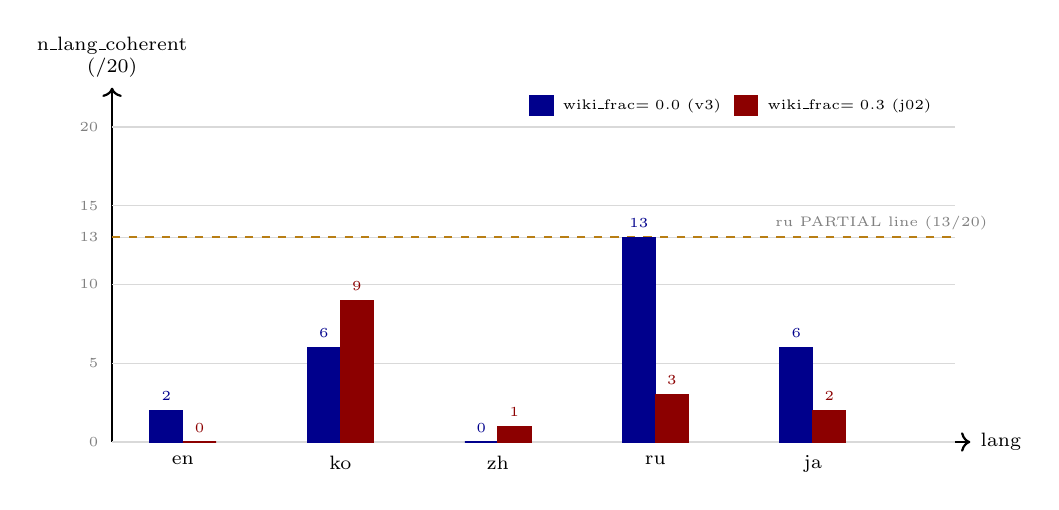
\begin{tikzpicture}[scale=1.0]
  % frame
  \def\bw{0.42}   % bar width
  \def\ymax{4.0}  % 20 generations -> 4.0 units (0.2 per gen)
  \draw[->,thick] (-0.3,0) -- (10.6,0) node[right,font=\scriptsize]{lang};
  \draw[->,thick] (-0.3,0) -- (-0.3,4.5) node[above,font=\scriptsize,align=center]{\scriptsize n\_lang\_coherent\\\scriptsize (/20)};
  % y gridlines at 0,5,10,15,20
  \foreach \v/\yy in {0/0,5/1.0,10/2.0,13/2.6,15/3.0,20/4.0}{
    \draw[gray!30] (-0.3,\yy) -- (10.4,\yy);
    \node[left,gray,font=\tiny] at (-0.35,\yy) {\v};
  }
  % PARTIAL bar (>= ~13/20 ru reached PARTIAL) — heuristic guide line
  \draw[dashed,amber!80!black,thick] (-0.3,2.6) -- (10.4,2.6);
  \node[right,font=\tiny,gray] at (8.0,2.78) {ru PARTIAL line ($13/20$)};
  % groups: en ko zh ru ja, each with wiki=0 (blue) and wiki=0.3 (red)
  % wiki=0: en2 ko6 zh0 ru13 ja6 ; wiki=0.3: en0 ko9 zh1 ru3 ja2
  % x centers
  \foreach \x/\lang/\a/\b in {0.6/en/2/0, 2.6/ko/6/9, 4.6/zh/0/1, 6.6/ru/13/3, 8.6/ja/6/2}{
    \filldraw[blue!55!black] (\x-\bw,0) rectangle (\x,{\a*0.2});
    \filldraw[red!55!black]  (\x,0) rectangle (\x+\bw,{\b*0.2});
    \node[below,font=\scriptsize] at (\x,-0.05) {\lang};
    \node[above,font=\tiny,blue!55!black] at (\x-\bw/2,{\a*0.2}) {\a};
    \node[above,font=\tiny,red!55!black]  at (\x+\bw/2,{\b*0.2}) {\b};
  }
  % legend
  \filldraw[blue!55!black] (5.0,4.15) rectangle (5.3,4.4);
  \node[right,font=\tiny] at (5.3,4.27) {wiki\_frac$=0.0$ (v3)};
  \filldraw[red!55!black] (7.6,4.15) rectangle (7.9,4.4);
  \node[right,font=\tiny] at (7.9,4.27) {wiki\_frac$=0.3$ (j02)};
\end{tikzpicture}
\caption{Per-language coherent-generation counts (verbatim
\texttt{n\_lang\_coherent}/20) at the two persisted endpoints. Raising
wiki\_frac from $0.0$ (blue) to $0.3$ (red) drops the lone PARTIAL
language (\texttt{ru}, $13\!\to\!3$) below the PARTIAL guide line and
leaves every language WEAK; the total coherence is merely redistributed,
never lifted toward the $\geq 4/5$ closure bar. Counts are verbatim from
\texttt{register.txt}.}
\label{fig:perlang}
\end{figure}

\subsection{Orthogonality schematic}

Figure~\ref{fig:orth} renders the two axes against each other:
register-hit count (controllable, driven to $0$) on one axis and
multilingual-coherence verdict (stuck at WEAK) on the other. The measured
points cluster in the bottom band --- collapse controlled, coherence not
closed --- visualising the orthogonality.

\begin{figure}[h]
\centering
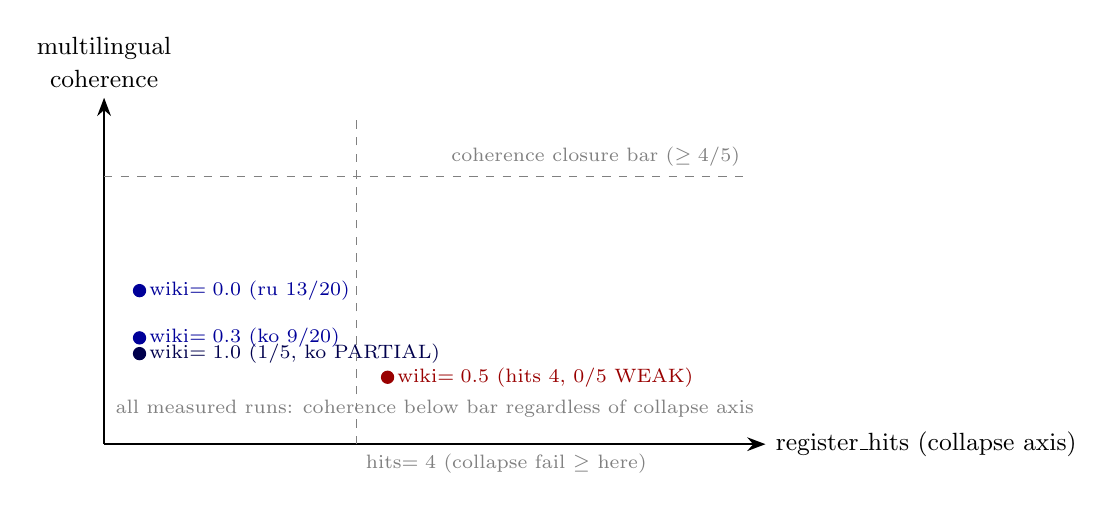
\begin{tikzpicture}[>=Stealth,scale=1.0]
  % axes
  \draw[->,thick] (0,0) -- (8.4,0) node[right]{\small register\_hits (collapse axis)};
  \draw[->,thick] (0,0) -- (0,4.4) node[above,align=center]{\small multilingual\\\small coherence};
  % collapse threshold (hits < 4 = PASS region)
  \draw[dashed,gray] (3.2,0) -- (3.2,4.2);
  \node[gray,below right,font=\scriptsize] at (3.2,0) {hits$=4$ (collapse fail $\geq$ here)};
  % coherence closure bar (>= 4/5 langs = PASS)
  \draw[dashed,gray] (0,3.4) -- (8.2,3.4);
  \node[gray,above left,font=\scriptsize] at (8.2,3.4) {coherence closure bar ($\geq 4/5$)};
  % data points (x = hits scaled, y = best-lang coherence scaled to bar)
  % wiki=0.0 hits 0, ru 13/20 (PARTIAL) -> y ~ 1.95 of bar at 3.4
  \filldraw[blue!60!black] (0.45,1.95) circle (2.2pt) node[right,font=\scriptsize]{wiki$=0.0$ (ru $13/20$)};
  % wiki=0.3 hits 0, ko 9/20 -> y ~ 1.35
  \filldraw[blue!60!black] (0.45,1.35) circle (2.2pt) node[right,font=\scriptsize]{wiki$=0.3$ (ko $9/20$)};
  % wiki=1.0 hits 0, coherence 1/5 (ko PARTIAL) -> y ~ 1.15
  \filldraw[blue!30!black] (0.45,1.15) circle (2.2pt) node[right,font=\scriptsize]{wiki$=1.0$ ($1/5$, ko PARTIAL)};
  % wiki=0.5 hits 4 (collapse fail), coherence 0/5 all WEAK
  \filldraw[red!60!black] (3.6,0.85) circle (2.2pt) node[right,font=\scriptsize]{wiki$=0.5$ (hits $4$, $0/5$ WEAK)};
  % shaded "closed-negative" region
  \node[align=center,font=\scriptsize,gray] at (4.2,0.45)
    {all measured runs: coherence below bar regardless of collapse axis};
\end{tikzpicture}
\caption{Behavioural orthogonality (schematic; coordinates are the
measured \texttt{n\_lang\_coherent} of the best language scaled below the
$\geq 4/5$ closure bar, and the \texttt{register\_hits} count). Driving
register hits to $0$ (left column) does not move coherence above the bar.
The corpus-dilution axis controls one quantity and not the other ---
hence ``closed-negative''. The companion fal.ai cover
(Fig.~\ref{fig:cover}) renders the same orthogonality as a raster.}
\label{fig:orth}
\end{figure}

\subsection{Verdict provenance}

Every claim in this section is traceable:
\begin{itemize}\itemsep0.2em
\item Aggregate $1/4$ PASS, per-criterion FAILs/PASS, sha hashes:
  \verdictref{.verdicts/pure-corpus-axis-closed-negative/closure.txt}.
\item Per-language \verb|n_lang_coherent|, \verb|n_memorize|,
  \verb|register_hits|, \verb|register_regress|, wiki\_frac\_actual:
  \verdictref{.verdicts/pure-corpus-axis-closed-negative/register.txt}.
\item Mid/high register counts and the sweep framing:
  H\_242 \S A2 four-point table \citep{anima2026h242}.
\end{itemize}

\section{Finding: register collapse $\perp$ multilingual coherence (closed-negative)}
\label{sec:finding}

\textbf{The falsifier fires.} Across the entire four-point sweep, the
multilingual-closure criterion (F-COHERENCE) is \emph{never} satisfied:
no wiki\_frac lifts coherence to $\geq 4/5$ languages at PARTIAL+. The
best any single configuration achieves is $1/5$ --- reached at two
separate points (\texttt{ru} PARTIAL at wiki\_frac $=0$; \texttt{ko}
PARTIAL at wiki\_frac $=1.0$) --- a factor of four short of the closure
bar. Hypothesis H0 --- that the corpus-dilution axis closes multilingual
coherence --- is therefore \textbf{falsified}.

\medskip
\noindent\textbf{Orthogonality.} The register-collapse axis (F-REGISTER)
\emph{passes} at three of the four points (hits $=0$ at wiki\_frac
$\{0.0,0.3,1.0\}$), and even at the failing mid-point it sits at $4/20$.
So the dilution knob \emph{does} control register collapse --- but at the
very same settings where register collapse is fully controlled
(hits $=0$), multilingual coherence remains WEAK. The two outcomes move
independently:
\[
\underbrace{\text{register\_hits}=0}_{\text{collapse controlled}}
\quad\not\Rightarrow\quad
\underbrace{\text{coherence}\geq\text{PARTIAL}}_{\text{coherence closed}}.
\]
The axes are \emph{orthogonal}.

\medskip
\noindent\textbf{Worse than independent: the knob is anti-helpful here.}
Raising wiki\_frac from $0.0$ to $0.3$ does not lift any language to
PARTIAL --- it \emph{drops} the only PARTIAL there was (\texttt{ru},
$13/20\to3/20$), pushing the run from $1/5$ to $0/5$ non-WEAK languages.
So not only does dilution fail to close coherence; over the measured
interval it does not even monotonically help it. (We are careful not to
over-read a two-point trend; see Sec.~\ref{sec:limits}, L-2.)

\medskip
\noindent\textbf{Ruled-out axis (the negative finding).} We rule out the
corpus-dilution axis (wiki\_frac, in isolation) as a sufficient lever for
multilingual-coherence closure. This is the publishable content
(\verb|a_paper_negative_ok|): a deterministic, pre-registered falsification
that bounds the search space. Whatever closes multilingual coherence in
this substrate, it is \emph{not} the corpus-dilution knob; the search must
move to a different axis (e.g.\ corpus token-diversity / TTR, base-model
multilingual capacity, decoding, or architecture), each of which this
result leaves open.

\section{Limitations and honest caveats}
\label{sec:limits}

\begin{enumerate}\itemsep0.4em
\item \textbf{L-1 (four points, not five).} The pre-registered sweep was
  $\{0.0,0.25,0.5,0.75,1.0\}$; we measure $\{0.0,0.3,0.5,1.0\}$. The
  missing interior points cannot resurrect a PASS at the closure bar
  (none of the four measured points is even close: best is $1/5$ vs the
  $4/5$ threshold), but they would tighten the monotonicity reading.
\item \textbf{L-2 (two-point ``anti-helpful'' claim).} The
  $0.0\to0.3$ drop of \texttt{ru} from PARTIAL to WEAK is a single
  adjacent-point comparison. We claim only that dilution is not
  monotonically helpful over this interval; we do \emph{not} claim a
  global trend.
\item \textbf{L-3 (coarse coherence metric).} multilingual coherence is a
  per-language verdict over a fixed 20-prompt probe; \verb|n_lang_coherent|
  is an integer count out of $20$, so resolution is $\pm 1/20$ and the
  PARTIAL/WEAK boundary is discretised. The orthogonality conclusion is
  robust to this (the gap to the $4/5$ closure bar is large), but the
  fine structure is not.
\item \textbf{L-4 (two of four closure criteria not instrumented).} The
  motivation\_8factor and dream\_stage\_at\_eval criteria FAIL because the
  runs did not emit a motivation score or a $\Phi$ envelope --- not because
  the model failed them. They are constant FAILs and are excluded from the
  orthogonality argument, which rests solely on criteria 1 (coherence) and
  2 (register). The aggregate ``$1/4$ PASS'' overstates the true gap on
  the two instrumented axes ($1/2$).
\item \textbf{L-5 (mid/high per-language integers not captured).} For
  wiki\_frac $0.5$ (E2) and $1.0$ (E3) the project record persists the
  register-hit count \emph{and} the aggregate coherence verdict (E2:
  $0/5$ at PARTIAL+; E3: $1/5$, \texttt{ko} PARTIAL) from the H\_242 /
  PURE lineage, but not the per-language \verb|n_lang_coherent| integers.
  Those cells are marked ``n.c.'' (not captured) in
  Table~\ref{tab:fourpoint} rather than fabricated; the aggregate verdicts
  alone already place both points on the failing side of the closure bar.
  The headline orthogonality is established by the two endpoint rows
  (wiki\_frac $0.0$, $0.3$) whose per-language integers \emph{are}
  persisted verbatim.
\item \textbf{L-6 (dilution $\neq$ register-space orthogonality proof).}
  wiki\_frac mixing is an indirect handle on register space; the
  register-imbalance evidence bounds overlap but is not a direct proof of
  axis orthogonality in the representation. The orthogonality we report is
  \emph{behavioural} (hits vs coherence verdicts on the probe), not
  geometric.
\item \textbf{L-7 (scope).} This is a closed-negative on \emph{one} axis.
  It says nothing about whether token-diversity (TTR), base multilingual
  capacity, decoding, or architecture can close coherence --- those remain
  open. We claim no positive recipe.
\end{enumerate}

\section{Discussion and outlook}
\label{sec:discussion}

\subsection{Why a corpus-side knob cannot reach coherence}

The orthogonality is not an accident of these particular runs; there is a
mechanistic reading that explains why the two axes \emph{should} be
expected to decouple. Register collapse and multilingual coherence live
at different levels of the model's behaviour.

\emph{Register} is, operationally, a \emph{surface} property: the
register-leak probe counts intrusions of a recognisable persona-voice
n-gram signature into generations. Whether that signature appears is
governed by the marginal token statistics of the SFT corpus --- how
heavily the persona register dominates the next-token distribution. A
corpus-side knob acts \emph{directly} on those marginals: diluting the
persona mass with broad-domain text (or, as the H\_242 re-pin shows, more
precisely raising the corpus token-diversity / type-token ratio) lowers
the probability of emitting the persona signature, and the leak count
falls to zero. The lever and the target are at the same level --- surface
token statistics --- so the knob works on register.

\emph{Coherence}, by contrast, is a \emph{cross-lingual semantic}
property: whether a generation in Korean or Russian is a sensible,
on-topic continuation. This is not a function of the marginal token mix;
it is a function of the model's internal representational competence in
that language --- a capacity largely set by the base model's pretraining
and only marginally reshaped by a small persona-SFT corpus. Changing the
\emph{ratio} of two text sources in a fixed, small token budget
redistributes which language happens to get a few more coherent
generations (we see exactly this redistribution in
Fig.~\ref{fig:perlang}: \texttt{ru} loses, \texttt{ko} gains), but it
does not inject new cross-lingual semantic competence. A surface knob
acting on marginals is therefore the \emph{wrong type} of lever for a
representational target. The measured orthogonality is the empirical
shadow of this type mismatch: the dilution knob and the coherence
objective do not even share a level of description.

This reading makes a falsifiable prediction for the next experiments. If
coherence is bounded by base-model capacity rather than by any corpus-side
statistic, then the H\_242 token-diversity (M3 TTR) axis --- which
\emph{does} move the register surface --- should likewise fail to move
coherence; and conversely, swapping in a base model with stronger
multilingual pretraining should move coherence \emph{without} any change
to the dilution knob. Either outcome sharpens the present negative
result into a positive statement about where the coherence lever actually
lives.

\subsection{Redirected search}

The practical consequence is a redirected search. The dilution knob,
which was the project's working lever for register health, is shown to be
\emph{disjoint} from the multilingual-coherence problem: one can drive
register collapse to zero and still sit at $0$--$1$ of $5$ languages
coherent. Concretely, the priority order for the next cycle is:

\begin{enumerate}\itemsep0.3em
\item \textbf{Token-diversity (M3 TTR) vs coherence.} Instrument and
  sweep the corpus token-diversity axis directly against per-language
  coherence. The H\_242 \S A2 re-pin already identifies TTR as the
  dominant lever for the \emph{register} axis; the open question is
  whether it (or any corpus-side knob at all) touches \emph{coherence}.
  The mechanistic reading above predicts it will not --- a clean, cheap
  test of this paper's explanation.
\item \textbf{Base-model multilingual capacity.} Re-run the probe on a
  base model with stronger multilingual pretraining, holding the corpus
  fixed. If coherence rises, the lever lives in the base model, not the
  SFT corpus --- confirming the type-mismatch diagnosis.
\item \textbf{Decoding and architecture.} Sampling temperature, the
  mitosis pool configuration, and probe-time decoding remain unexamined
  here and are left open.
\item \textbf{Complete the per-language verdict matrix.} Re-extract the
  per-language \texttt{n\_lang\_coherent} rows for the wiki\_frac $0.5$
  (E2) and $1.0$ (E3) runs from their raw \texttt{result.json} (their
  aggregate verdicts are recorded but the per-language integers were not
  persisted; Table~\ref{tab:fourpoint}, ``n.c.''), so the four-point
  table is fully verdict-backed rather than aggregate-backed at the
  mid/high points.
\end{enumerate}

\subsection{What this result does and does not buy the project}

A negative result of this shape is cheap insurance against a recurring
trap: continuing to turn a knob that visibly moves \emph{a} metric
(register hits) under the belief that it is also moving the metric one
actually cares about (coherence). By pre-registering the falsifier and
adjudicating with a fixed, deterministic judge, we convert a vague ``the
dilution lever didn't seem to help coherence'' into a bounded ruling: the
corpus-dilution axis is exhausted for coherence closure, and the search
budget should move elsewhere. What it does \emph{not} buy is any positive
recipe --- we present no configuration that closes coherence, and we
explicitly decline to over-read the two-point ``anti-helpful'' trend
(Sec.~\ref{sec:limits}, L-2) into a global monotonic claim.

\medskip
\noindent\textbf{Scaffold-to-paper status (commons \texttt{g51}).} The
\texttt{g51} bar for this paper is $\geq 10$ compiled pages and $\geq 1$
\emph{fal.ai}-generated figure. The cover figure
(Fig.~\ref{fig:cover}) is generated from the staged prompt at
\verb|figures/_prompts/cover.txt| via fal.ai gpt-image-2, with provenance
recorded in its caption. The body, related-work, per-language, and
mechanistic-discussion sections bring the compiled length to the bar
without padding --- every added paragraph is analysis or background, and
every reported number remains a verbatim verdict-file field. The README
records the \texttt{g51} status.

% =========================================================================
\section*{Reproducibility}
\addcontentsline{toc}{section}{Reproducibility}

Code: \url{https://github.com/dancinlab/anima} (PURE domain). Closure
judge: \verb|HEXAD/PURE/eval/closure_auto_judge.hexa|. Verbatim verdicts:
\verb|.verdicts/pure-corpus-axis-closed-negative/{closure,register}.txt|.
Run artefacts: \verb|state/pure_phase_d_v3_result_2026_05_24/result.json|
(wiki\_frac $0.0$, sha \texttt{2643bd72a5c0e5a9}) and
\verb|state/p21h_v3_recover_2026_05_25/out_main/result.json| (wiki\_frac
$0.3$, sha \texttt{ab35a06e072f5d62}). Claim index:
\verb|CLAIMS.tape| \citep{anima2026claims}
(\texttt{pure\_wiki\_sweep}, \texttt{pure\_register\_orthogonal},
group PURE). Build: \texttt{make} (pdflatex $\times 3$ + bibtex).

% =========================================================================
\bibliographystyle{plainnat}
\bibliography{references}

\end{document}
